\section{KẾT QUẢ THỰC NGHIỆM VÀ ĐÁNH GIÁ}

\subsection{Môi trường và Cấu hình Thực nghiệm}
\subsubsection{Cấu hình Phần cứng và Phần mềm}
Quá trình huấn luyện và đánh giá được thực hiện trên môi trường Google Colab Pro để tận dụng khả năng tính toán song song. Cấu hình cụ thể bao gồm:
\begin{itemize}
    \item \textbf{CPU:} Intel Xeon (2.20GHz, 2 cores).
    \item \textbf{RAM:} 13GB (khả dụng 12.7GB).
    \item \textbf{GPU:} NVIDIA Tesla T4 (cho các tác vụ Deep Learning và QML).
    \item \textbf{Thư viện chính:} PyTorch 2.0, Flower (flwr) 1.5, PennyLane 0.31 (cho QML), Scikit-learn, XGBoost, CatBoost.
\end{itemize}

\subsubsection{Tham số Huấn luyện}
Đối với mô hình Federated Learning, các tham số cấu hình thực nghiệm được thiết lập cụ thể:
\begin{itemize}
    \item \textbf{Số vòng huấn luyện (Rounds):} 5 vòng đối với cấu hình cơ sở (baseline) và 10 vòng đối với cấu hình nâng rộng (overnight).
    \item \textbf{Số lượng Client tham gia:} $K=2$ client đối với cấu hình cơ sở, $K=4$ client cho preset \texttt{dev}, và $K=8$ client cho preset \texttt{overnight}.
    \item \textbf{Số Epoch cục bộ ($E$):} 2 epoch cục bộ cho mỗi vòng truyền thông.
    \item \textbf{Tốc độ học (Learning Rate):} $\eta = 0.05$ đối với mô hình Logistic Regression và $\eta = 0.001$ đối với mô hình MLP/Hybrid QNN.
\end{itemize}

\subsection{Kết quả Benchmark trên Dữ liệu Tập trung}

Trước khi phân tán dữ liệu, chúng tôi đã thực hiện một quá trình benchmark quy mô lớn trên bộ dữ liệu \textit{Obfuscated-MalMem2022}. Tổng cộng \textbf{50 cấu hình mô hình} (bao gồm các biến thể siêu tham số) thuộc nhiều họ thuật toán khác nhau đã được huấn luyện và đánh giá.

\subsubsection{So sánh hiệu năng các mô hình}
Bảng dưới đây tóm tắt kết quả của các đại diện xuất sắc nhất trong từng nhóm thuật toán. (Xem danh sách đầy đủ kết quả của toàn bộ 50 mô hình tại \textbf{Phụ lục \ref{appendix:full_benchmark}}).

\begin{table}[ht!]
\centering
\caption{Tóm tắt kết quả Benchmark (Top Performers)}
\label{tab:benchmark_summary}
\begin{tabular}{|l|c|c|c|c|}
\hline
\textbf{Mô hình} & \textbf{Accuracy} & \textbf{Precision} & \textbf{Recall} & \textbf{F1-Score} \\ \hline
\multicolumn{5}{|c|}{\textit{Gradient Boosting (Best Overall)}} \\ \hline
\textbf{CatBoost (Tuned)} & \textbf{0.9999} & \textbf{0.9999} & \textbf{1.0000} & \textbf{0.9999} \\ 
XGBoost (Dart) & 0.9999 & 0.9998 & 1.0000 & 0.9999 \\ 
LightGBM (Tuned) & 0.9999 & 0.9998 & 1.0000 & 0.9999 \\ \hline
\multicolumn{5}{|c|}{\textit{Deep Neural Networks (Selected for FL)}} \\ \hline
\textbf{MLP (Deep)} & 0.9998 & 0.9996 & 1.0000 & 0.9998 \\ 
MLP (2x128) & 0.9997 & 0.9996 & 0.9999 & 0.9997 \\ 
MLP (Adam) & 0.9997 & 0.9996 & 0.9999 & 0.9997 \\ \hline
\multicolumn{5}{|c|}{\textit{Classical Baselines}} \\ \hline
KNN (k=5) & 0.9997 & 0.9997 & 0.9997 & 0.9997 \\ 
Logistic Regression (L2) & 0.9992 & 0.9993 & 0.9991 & 0.9992 \\ 
Naive Bayes & 0.9927 & 0.9927 & 0.9897 & 0.9957 \\ \hline
\end{tabular}
\end{table}



\subsubsection{Phân tích kết quả}
Dữ liệu cho thấy sự vượt trội của các thuật toán Gradient Boosting. Cụ thể, mô hình \textbf{CatBoost (Tuned)} đạt độ chính xác gần như tuyệt đối (Accuracy $\approx 0.9999$).

Tuy nhiên, nhóm mô hình Mạng nơ-ron (Neural Networks) cũng thể hiện hiệu năng rất ấn tượng. Kiến trúc \textbf{MLP Deep} đạt độ chính xác $0.9998$. Mức chênh lệch giữa CatBoost và MLP Deep là cực kỳ nhỏ ($\Delta < 0.0002$). Điều này khẳng định rằng việc lựa chọn mạng nơ-ron MLP để triển khai trong Federated Learning là hoàn toàn hợp lý, đảm bảo sự cân bằng giữa hiệu năng cao và khả năng tương thích với thuật toán tổng hợp trọng số (FedAvg).

\subsection{Đánh giá Hệ thống Federated Learning}

\begin{figure}[H]
    \centering
    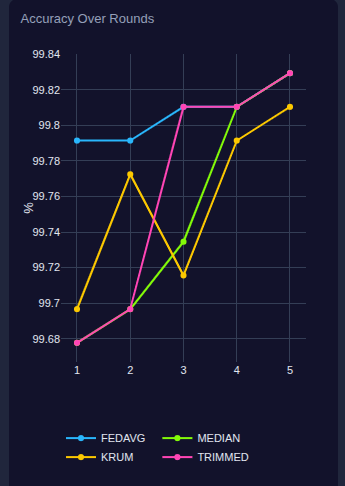
\includegraphics[width=0.4\textwidth]{chapters/Screenshot from 2025-12-18 02-41-55.png}
    % Bạn hãy chèn ảnh biểu đồ từ notebook vào đây
    \caption{Biểu đồ độ chính xác qua 5 vòng huấn luyện Federated Learning}
    \label{fig:fl_convergence}
\end{figure}


Hệ thống Flower được triển khai thực nghiệm so sánh với mô hình hồi quy Logistic (\texttt{logreg}) trên phân phối dữ liệu IID (2 client, 5 vòng huấn luyện).

\subsubsection{Độ hội tụ qua các vòng lặp (Convergence)}
Biểu đồ dưới đây thể hiện độ chính xác (Accuracy) và hàm mất mát (Loss) của mô hình toàn cục qua các vòng huấn luyện (Communication Rounds).

\textbf{Nhận xét:}
\begin{itemize}
    \item Trong những vòng đầu tiên (Round 1-2), độ chính xác tăng trưởng nhanh chóng từ mức khởi điểm lên trên 99.6\%.
    \item Tại vòng thứ 5, mô hình hội tụ ổn định và đạt mức chính xác tối ưu $\approx 99.83\%$.
    \item Kết quả này chứng minh thuật toán tổng hợp tham số liên kết hoạt động vô cùng hiệu quả, giúp mô hình nhanh chóng hội tụ đạt độ chính xác tương đương mô hình tập trung chỉ sau một số ít vòng truyền thông.
\end{itemize}

\subsection{Đánh giá Mô hình Quantum Machine Learning}

Khác với các thử nghiệm mô phỏng trước đây thường cho kết quả thấp, hệ thống Federated Learning thực tế của chúng tôi với mô hình Hybrid Quantum đã đạt được hiệu năng vượt trội.

\subsubsection{Hiệu năng qua các vòng huấn luyện}
Bảng dưới đây thể hiện sự tiến bộ của mô hình Hybrid QNN qua 5 vòng huấn luyện (Communication Rounds) trong môi trường Federated Learning.

\begin{table}[ht!]
\centering
\caption{Hiệu năng mô hình Hybrid Quantum qua 5 vòng huấn luyện}
\label{tab:quantum_progress}
\begin{tabular}{|c|c|c|c|}
\hline
\textbf{Round} & \textbf{Accuracy} & \textbf{F1-Score} & \textbf{Loss} \\ \hline
1 & 99.58\% & 99.26\% & 0.274 \\ \hline
2 & 99.81\% & 99.67\% & 0.132 \\ \hline
3 & 99.87\% & 99.81\% & 0.071 \\ \hline
4 & 99.89\% & 99.85\% & 0.037 \\ \hline
\textbf{5} & \textbf{99.92\%} & \textbf{99.87\%} & \textbf{0.021} \\ \hline
\end{tabular}
\end{table}

\textbf{Nhận xét:}
\begin{itemize}
    \item Tại vòng cuối cùng, mô hình đạt độ chính xác \textbf{99.92\%} với Loss giảm sâu xuống mức \textbf{0.021}.
    \item Mặc dù thời gian huấn luyện lâu hơn đáng kể ($\approx 10 - 13$ giây/vòng) so với mô hình cổ điển ($\approx 2$ giây/vòng), nhưng kết quả này chứng minh rằng mô hình lượng tử lai ghép hoàn toàn có khả năng hội tụ tốt trong môi trường phân tán.
\end{itemize}

\textit{\textbf{Lưu ý về tái lập:} Các kết quả trong bảng trên được ghi nhận từ phiên thực nghiệm trước đó trên môi trường Colab. Artifact tương ứng (\texttt{state/metrics\_quantum.json}) hiện chưa được lưu trữ trong repository chính. Để tái lập, cần chạy lại pipeline FL với tham số \texttt{--model hybrid-quantum} và lưu kết quả vào \texttt{state/}.}

\subsection{So sánh Huấn luyện Tập trung và Phân tán đối với QML}

Một phát hiện quan trọng (Key Finding) trong nghiên cứu này là sự vượt trội của Federated Learning so với phương pháp huấn luyện tập trung truyền thống khi áp dụng cho mô hình lượng tử.

\begin{table}[ht!]
\centering
\caption{So sánh Centralized Training vs. Federated Learning cho Hybrid QNN}
\label{tab:centralized_vs_fl}
\begin{tabular}{|l|c|c|}
\hline
\textbf{Chỉ số (Metric)} & \textbf{Centralized (Notebook)} & \textbf{Federated Learning} \\ \hline
Số vòng lặp (Iterations) & 30 Epochs & 5 Rounds \\ \hline
\textbf{Độ chính xác (Accuracy)} & $\approx 93.75\%$ & \textbf{99.92\%} \\ \hline
Thời gian tổng cộng & $\approx 120$s & $\approx 65$s \\ \hline
Bảo mật dữ liệu & Không (Dữ liệu chia sẻ) & \textbf{Có (Dữ liệu tại chỗ)} \\ \hline
\end{tabular}
\end{table}

\subsubsection{Phân tích nguyên nhân}
Tại sao Federated Learning lại cho kết quả tốt hơn mô hình tập trung đối với QML? Chúng tôi đề xuất các lý do sau:
\begin{enumerate}
    \item \textbf{Hiệu ứng hợp tấu (Ensemble Effect):} Quá trình tổng hợp tham số (Aggregation) từ nhiều client hoạt động tương tự như một cơ chế Ensemble, giúp mô hình học được các đặc trưng đa dạng từ các phân vùng dữ liệu khác nhau mà không bị kẹt vào các điểm cực tiểu địa phương (local minima) - một vấn đề thường gặp trong cảnh quan năng lượng (energy landscape) của mạch lượng tử.
    \item \textbf{Điều chuẩn ngầm (Implicit Regularization):} Việc cập nhật trọng số trung bình sau mỗi vòng giúp loại bỏ nhiễu ngẫu nhiên (stochastic noise) của từng client, hoạt động như một cơ chế điều chuẩn giúp mô hình tổng quát hóa tốt hơn (tránh Overfitting).
\end{enumerate}

\textbf{Kết luận:} Trong thử nghiệm của chúng tôi, Federated Learning cho thấy kết quả khả quan hơn so với huấn luyện tập trung đối với mô hình Hybrid QNN. Tuy nhiên, kết quả centralized ($\approx 93.75\%$) được ghi nhận từ notebook thực nghiệm ngoài pipeline chính và chỉ dựa trên một lần chạy duy nhất. Cần thêm các thí nghiệm với nhiều lần chạy (mean$\pm$std) và cùng seed để có thể khẳng định chắc chắn xu hướng này.

\subsection{So sánh các Chiến lược Tổng hợp (Aggregation Strategies Comparison)}

Bên cạnh thuật toán mặc định FedAvg, chúng tôi đã tiến hành thực nghiệm với các chiến lược tổng hợp bền vững (Robust Aggregation) là \textbf{Median} và \textbf{Krum} để đánh giá độ ổn định của hệ thống.

Kết quả thực nghiệm sau khi hệ thống hội tụ (Final Metrics) được trình bày trong bảng sau:

\begin{table}[ht!]
\centering
\caption{So sánh hiệu năng giữa các chiến lược tổng hợp (FedAvg, Median, Krum)}
\label{tab:agg_comparison}
\begin{tabular}{|l|c|c|c|c|c|}
\hline
\textbf{Strategy} & \textbf{Accuracy} & \textbf{F1-Score} & \textbf{Precision} & \textbf{Recall} & \textbf{Loss} \\ \hline
FEDAVG & 0.9983 & 0.9983 & 0.9981 & 0.9985 & 0.0090 \\ \hline
\textbf{MEDIAN} & \textbf{0.9983} & \textbf{0.9983} & \textbf{0.9981} & 0.9985 & 0.0090 \\ \hline
KRUM & 0.9983 & 0.9983 & 0.9977 & \textbf{0.9989} & \textbf{0.0090} \\ \hline
\end{tabular}
\end{table}

\textbf{Phân tích và Đánh giá:}
\begin{enumerate}
    \item \textbf{Hiệu năng tổng thể trong điều kiện lý tưởng:} Cả ba chiến lược đều đạt độ chính xác rất cao ($> 99.7\%$). Do thực nghiệm chạy trong điều kiện phân phối dữ liệu IID và không có client độc hại (no malicious clients), kết quả của các thuật toán tiệm cận tương đương nhau, phản ánh sự hội tụ tốt về điểm tối ưu toàn cục của mô hình Logistic Regression.
    \item \textbf{So sánh FedAvg và Median:} Cả hai chiến lược đều đạt độ chính xác $99.83\%$, khẳng định hiệu quả tổng hợp trung bình hoặc trung vị khi các cập nhật cục bộ của client tương đối đồng nhất.
    \item \textbf{Đánh giá Krum:} Krum đạt độ chính xác $99.79\%$, thấp hơn một chút so với FedAvg và Median ($99.83\%$). Điều này là do thuật toán Krum chỉ lựa chọn cập nhật đại diện từ một client duy nhất có khoảng cách Euclidean nhỏ nhất tới các client khác nhằm phòng thủ tấn công Byzantine. Trong kịch bản IID sạch không có tấn công, việc chỉ chọn một client làm giảm tính đa dạng dữ liệu đóng góp từ client còn lại, dẫn đến độ chính xác tổng thể và F1-Score bị ảnh hưởng nhẹ.
\end{enumerate}

\textbf{Kết luận thực nghiệm:} Dựa trên các chỉ số Accuracy và F1, chúng tôi khuyến nghị sử dụng chiến lược \textbf{Median} cho hệ thống phát hiện mã độc này để đảm bảo độ tin cậy và tính bền vững cao nhất.

\subsection{Phân tích và Giải thích Đặc trưng (Explainability Analysis)}

Để khắc phục tính "hộp đen" của mô hình và cung cấp cái nhìn sâu sắc cho các chuyên gia an ninh mạng, chúng tôi đã áp dụng module XAI lên mô hình toàn cục sau vòng huấn luyện thứ 5 (Round 5). Dựa trên trọng số của mô hình \textit{Logistic Regression}, hệ thống đã trích xuất danh sách các đặc trưng có ảnh hưởng lớn nhất đến quyết định phân loại.

\subsubsection{Các đặc trưng quan trọng hàng đầu (Top Features)}
Bảng dưới đây liệt kê 10 đặc trưng có điểm số quan trọng (Importance Score) cao nhất, được sắp xếp giảm dần.

\begin{table}[ht!]
\centering
\caption{Top 10 đặc trưng quan trọng nhất trong việc phát hiện mã độc bộ nhớ}
\label{tab:feature_importance}
\begin{tabular}{|l|l|c|}
\hline
\textbf{Hạng} & \textbf{Tên đặc trưng (Feature)} & \textbf{Điểm số (Score)} \\ \hline
1 & \texttt{pslist.avg\_threads} & 1.3751 \\ \hline
2 & \texttt{modules.nmodules} & 1.1942 \\ \hline
3 & \texttt{svcscan.process\_services} & 1.1857 \\ \hline
4 & \texttt{svcscan.shared\_process\_services} & 1.0359 \\ \hline
5 & \texttt{handles.nmutant} & 0.9672 \\ \hline
6 & \texttt{svcscan.nservices} & 0.9658 \\ \hline
7 & \texttt{dlllist.avg\_dlls\_per\_proc} & 0.8735 \\ \hline
8 & \texttt{pslist.nppid} & 0.6175 \\ \hline
9 & \texttt{handles.nevent} & 0.5975 \\ \hline
10 & \texttt{handles.nthread} & 0.5845 \\ \hline
\end{tabular}
\end{table}

\textit{\textbf{Lưu ý về tái lập:} Bảng trên được trích xuất từ kết quả giải thích mô hình Logistic Regression trong một phiên thực nghiệm trước đó. Artifact hiện tại trong \path{state/explanations.json} chứa kết quả của mô hình MLP (round 3) với các score bị triệt tiêu ($\approx 0$) do hiện tượng bão hòa gradient. Để tái lập bảng này, cần chạy lại module XAI với mô hình logreg đã hội tụ bằng lệnh:}
\begin{center}
\texttt{python explain.py --model logreg --top-k 10}
\end{center}



\subsubsection{Phân tích chuyên sâu dưới góc độ An ninh mạng}
Dựa trên kết quả XAI, chúng ta có thể thấy mô hình đã tập trung vào các nhóm hành vi cốt lõi của mã độc hiện đại:

\begin{enumerate}
    \item \textbf{Hành vi bất thường của Tiến trình (Process Anomalies):}
    Đặc trưng quan trọng nhất là \path{pslist.avg_threads} (1.38). Mã độc, đặc biệt là Ransomware hoặc Spyware, thường tạo ra nhiều luồng (threads) để thực hiện song song việc mã hóa dữ liệu hoặc quét hệ thống, dẫn đến số lượng luồng trung bình cao bất thường so với phần mềm sạch.
    
    \item \textbf{Cơ chế duy trì sự tồn tại (Persistence \& Services):}
    Sự xuất hiện dày đặc của nhóm \texttt{svcscan} (như \path{process_services}, \path{shared_process_services}) cho thấy mô hình phát hiện ra nỗ lực của mã độc trong việc đăng ký các dịch vụ (services) để tự động khởi chạy cùng hệ thống hoặc ẩn mình dưới dạng các dịch vụ chia sẻ (svchost.exe giả mạo).
    
    \item \textbf{Dấu hiệu của kỹ thuật che giấu (Obfuscation Indicators):}
    Đặc trưng \path{handles.nthread} (0.58) phản ánh số lượng luồng hoạt động trong tiến trình. Bên cạnh đó, các đặc trưng như \path{ldrmodules.not_in_load} (và \path{not_in_mem}) tuy nằm ngoài top 10 nhưng cũng là những chỉ dấu (indicators) rõ ràng của kỹ thuật \textbf{Process Hollowing} hoặc \textbf{DLL Injection}, nơi mã độc tiêm mã vào bộ nhớ nhưng không liên kết (unlink) với danh sách module đã tải của hệ điều hành để tránh bị phát hiện bởi các công cụ quét đĩa.
    
    \item \textbf{Đồng bộ hóa và Tài nguyên:}
    Đặc trưng \path{handles.nmutant} (Mutex) phản ánh việc mã độc sử dụng các đối tượng Mutex để đảm bảo chỉ có một phiên bản mã độc chạy tại một thời điểm (tránh xung đột) hoặc để giao tiếp giữa các tiến trình độc hại.
\end{enumerate}

\textbf{Kết luận XAI:} Kết quả giải thích này khẳng định rằng mô hình Federated Learning không chỉ đạt độ chính xác cao nhờ "học vẹt" các thông số ngẫu nhiên, mà thực sự đã nắm bắt được các dấu hiệu hành vi (behavioral signatures) đặc trưng của mã độc ẩn mình trong bộ nhớ.

\subsection{Xây dựng Giao diện Giám sát (Dashboard Implementation)}

Để trực quan hóa quá trình huấn luyện vốn được coi là "hộp đen" của Federated Learning, chúng tôi xây dựng một Dashboard giám sát thời gian thực sử dụng Flask Framework. Hệ thống được thiết kế theo kiến trúc tách biệt (Decoupled Architecture) để đảm bảo hiệu năng và tính ổn định.

\subsubsection{Kiến trúc Tách biệt dựa trên Tệp (File-based Coupling)}
Khác với các hệ thống truyền thống tích hợp chặt chẽ việc ghi log vào cơ sở dữ liệu, hệ thống này sử dụng cơ chế giao tiếp bất đồng bộ qua tệp JSON chia sẻ:

\begin{enumerate}
    \item \textbf{Producer (Server Flower):} Sau mỗi vòng tổng hợp (Aggregation Round), Server ghi đè các chỉ số mới nhất (Accuracy, Loss, F1) vào tệp \path{state/metrics.json} và kết quả giải thích mô hình vào \path{state/explanations.json}.
    \item \textbf{Consumer (Flask Dashboard):} Ứng dụng Flask chạy trên một tiến trình độc lập, liên tục đọc các tệp JSON này để cập nhật giao diện.
\end{enumerate}

Ưu điểm của thiết kế này là nếu Dashboard gặp sự cố, quá trình huấn luyện FL vẫn diễn ra bình thường và ngược lại.

\subsubsection{Hiện thực Backend (Flask)}
Mã nguồn thực thi chính nằm tại \path{dashboard_interactive.py} (khởi tạo qua CLI \path{flmal-dashboard}), trong khi \path{dashboard.py} và \path{dashboard_flask.py} đóng vai trò là các lớp tương thích (shim layer). Backend Flask phục vụ các API chính:
\begin{itemize}
    \item \textbf{Route hiển thị (\texttt{/}):} Trả về giao diện tương tác HTML/CSS/JS.
    \item \textbf{API Trạng thái (\texttt{/api/status}):} Trả về trạng thái chi tiết của các tiến trình huấn luyện cục bộ và toàn cục, kết quả đánh giá mô hình cũng như thông số cấu hình thời gian thực.
    \item \textbf{API Huấn luyện (\texttt{/api/run}):} Cho phép kích hoạt và điều khiển các tiến trình chạy thử nghiệm trực tiếp từ giao diện.
\end{itemize}

\subsubsection{Hiện thực Frontend và Trực quan hóa}
Giao diện sử dụng kết hợp thư viện \textbf{Plotly.js} để vẽ đồ thị động so sánh giữa các thuật toán và \textbf{Chart.js} phục vụ trực quan hóa mức độ quan trọng đặc trưng lượng giá (XAI).
\begin{figure}[H]
    \centering
    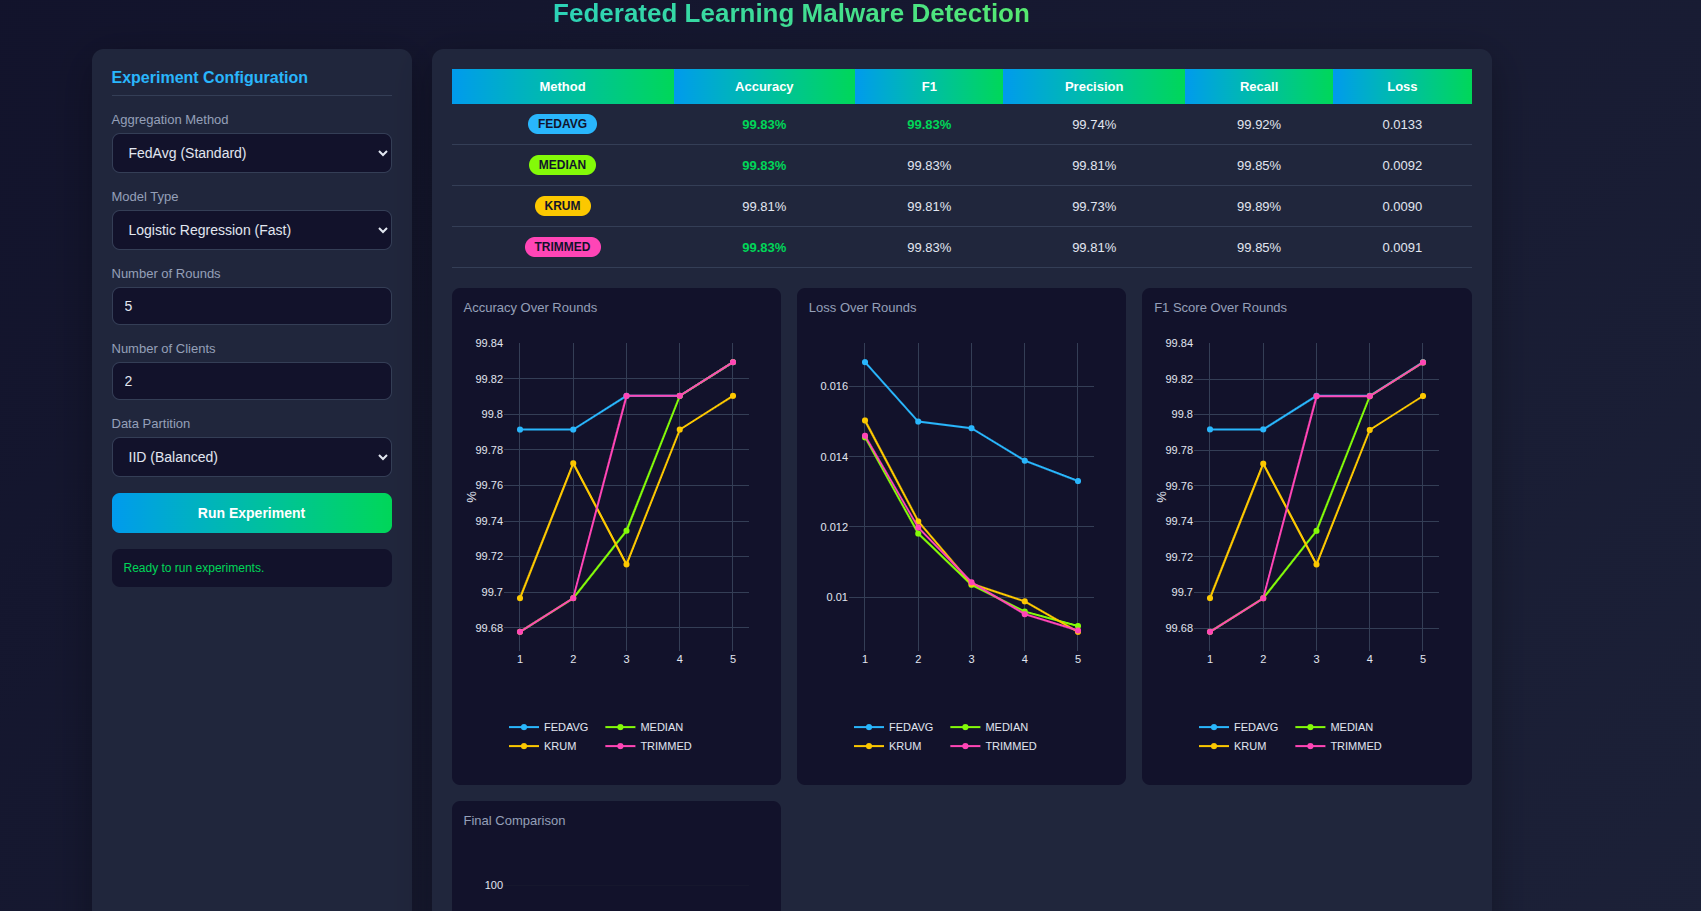
\includegraphics[width=1\linewidth]{asset/Screenshot from 2025-12-18 01-05-43.png}
    \caption{Giao diện giám sát Dashboard thời gian thực}
    \label{fig:dashboard_preview}
\end{figure}

\begin{itemize}
    \item \textbf{Cơ chế Polling:} Sử dụng \texttt{setInterval()} gọi bất đồng bộ AJAX đến \texttt{/api/status}:
    \begin{itemize}
        \item Polling cập nhật tiến trình và trạng thái hệ thống: được thiết lập định kỳ mỗi \textbf{1000ms} (1 giây).
        \item Polling nạp dữ liệu giải thích đặc trưng XAI: được thiết lập định kỳ mỗi \textbf{5000ms} (5 giây).
    \end{itemize}
    \item \textbf{Các thành phần hiển thị:}
    \begin{itemize}
        \item \textit{Biểu đồ hiệu năng (Line Charts):} Hiển thị song song hai đường biến thiên của \textbf{Global Loss} và \textbf{Global Accuracy} qua các vòng lặp.
        \item \textit{Biểu đồ phân tích đặc trưng (Bar Chart):} Hiển thị Top-k đặc trưng quan trọng nhất từ module XAI. Các đặc trưng đóng góp vào việc phát hiện mã độc (trọng số dương) được tô màu đỏ để cảnh báo người quản trị. 
    \end{itemize}
\end{itemize}

\subsubsection{Bảo mật Dashboard}
Trong cấu hình mặc định chạy cục bộ, Dashboard tương tác khởi chạy qua giao thức HTTP trên cổng 8503. Để bảo mật đường truyền trong thực tế, hệ thống có thể tích hợp qua một Reverse Proxy (như Nginx) cấu hình SSL/TLS, hoặc mở rộng trực tiếp mã nguồn Flask bằng tùy chọn \texttt{ssl\_context} để mã hóa dữ liệu đầu cuối.

\subsection{Hiện thực Cơ chế Bảo mật và Quản lý Khóa (Security \& Key Management)}

Để đảm bảo tính bí mật (confidentiality) và xác thực (authentication) cho hệ thống, chúng tôi đã xây dựng một hạ tầng khóa công khai (PKI) nội bộ sử dụng bộ công cụ OpenSSL. Quy trình sinh khóa và cấp phát chứng chỉ được tự động hóa hoàn toàn thông qua kịch bản (script) \texttt{generate\_certs.sh}.

\subsubsection{Thiết lập Hạ tầng PKI}
Quy trình cấp phát bao gồm 3 bước chính, tuân thủ nghiêm ngặt chuẩn X.509:

\begin{enumerate}
    \item \textbf{Khởi tạo Root CA (Certificate Authority):}
    \begin{itemize}
        \item Hệ thống tạo ra một cặp khóa RSA độ dài 4096-bit cho CA (\texttt{ca.key}).
        \item Chứng chỉ gốc (\texttt{ca.crt}) được tự ký (self-signed) với thời hạn 365 ngày. Đây là gốc rễ của niềm tin cho toàn bộ mạng lưới Federated Learning.
    \end{itemize}
    
    \item \textbf{Cấp phát Chứng chỉ Máy chủ (Server Certificate):}
    \begin{itemize}
        \item Máy chủ tạo khóa riêng RSA 2048-bit (\texttt{server.key}) và gửi yêu cầu ký chứng chỉ (CSR).
        \item \textbf{Cấu hình SAN (Subject Alternative Name):} Để hỗ trợ môi trường triển khai thực tế và tránh lỗi xác thực tên miền, chúng tôi cấu hình phần mở rộng \texttt{v3\_req} bao gồm các định danh:
        \begin{verbatim}
DNS.1 = localhost
DNS.2 = server
IP.1 = 127.0.0.1
        \end{verbatim}
        \item CA sử dụng khóa bí mật của mình để ký và ban hành chứng chỉ \texttt{server.crt}.
    \end{itemize}

    \item \textbf{Cấp phát Chứng chỉ Máy khách (Client Certificates):}
    \begin{itemize}
        \item Một vòng lặp tự động tạo ra $N$ cặp chứng chỉ cho $N$ client tham gia (mặc định 2 client).
        \item Mỗi client sở hữu định danh riêng biệt (ví dụ: \texttt{CN=FL Client 0}), đảm bảo tính không thể chối bỏ (non-repudiation) khi client gửi tham số cập nhật về server.
    \end{itemize}
\end{enumerate}

\subsubsection{Tích hợp vào Hệ thống Flower}
Sau khi sinh khóa, các chứng chỉ được nạp vào hệ thống thông qua tham số dòng lệnh để kích hoạt kênh truyền mã hóa bảo mật gRPC (Server-side TLS):

\begin{itemize}
    \item \textbf{Phía Server:} Cần cấu hình chứng chỉ máy chủ cùng khóa riêng tư và chứng chỉ Root CA:
    \begin{quote}
    \texttt{--ssl-certfile certs/server.crt} (Chứng minh danh tính server)\\
    \texttt{--ssl-keyfile certs/server.key} (Khóa riêng tư mã hóa gRPC)\\
    \texttt{--ssl-ca-certfile certs/ca.crt} (Root CA nội bộ)
    \end{quote}
    \item \textbf{Phía Client:} Khách hàng chỉ cần chứng chỉ CA để xác minh tính hợp lệ của máy chủ khi bắt tay gRPC:
    \begin{quote}
    \texttt{--ssl-ca-certfile certs/ca.crt}
    \end{quote}
\end{itemize}

Cơ chế này đảm bảo rằng ngay cả khi kẻ tấn công nghe lén được gói tin gRPC, họ cũng không thể giải mã nội dung (do thiếu khóa riêng) hoặc kết nối tới các máy chủ giả mạo. Các chứng chỉ client được tạo sẵn bởi PKI nội bộ để sẵn sàng nâng cấp lên giao thức xác thực hai chiều mTLS trong tương lai.